
\documentclass[aspectratio=169,11pt]{beamer}

% Compile with: pdflatex eer_model_beamer_pdflatex.tex
\usepackage[utf8]{inputenc}
\usepackage[T5]{fontenc}
\usepackage[vietnamese]{babel}
\usepackage{amsmath,amssymb}
\usepackage{booktabs,tabularx,array,multicol}
\usepackage{tikz}
\usetikzlibrary{positioning,arrows.meta,shapes.geometric,fit,calc}
\usepackage{listings}
\usepackage{xcolor}
\usepackage{graphicx}

\usetheme{Madrid}
\usecolortheme{default}
\setbeamertemplate{navigation symbols}{}
\setbeamertemplate{caption}[numbered]

\definecolor{NEUBlue}{RGB}{0,65,130}
\definecolor{NEULight}{RGB}{235,244,252}
\definecolor{NEUOrange}{RGB}{232,127,38}
\setbeamercolor{structure}{fg=NEUBlue}
\setbeamercolor{frametitle}{fg=white,bg=NEUBlue}
\setbeamercolor{title}{fg=white,bg=NEUBlue}
\setbeamercolor{block title}{fg=white,bg=NEUBlue}
\setbeamercolor{block body}{bg=NEULight,fg=black}
\setbeamercolor{alerted text}{fg=NEUOrange}

\lstdefinestyle{sqlstyle}{
    language=SQL,
    basicstyle=\ttfamily\scriptsize,
    keywordstyle=\bfseries\color{NEUBlue},
    commentstyle=\itshape\color{gray},
    stringstyle=\color{NEUOrange},
    showstringspaces=false,
    breaklines=true,
    columns=fullflexible,
    frame=single,
    rulecolor=\color{NEUBlue!30},
    xleftmargin=1mm,
    xrightmargin=1mm
}
\lstset{style=sqlstyle}

\newcommand{\concept}[1]{\textcolor{NEUBlue}{\textbf{#1}}}
\newcommand{\codeword}[1]{\texttt{#1}}

\title[Bài giảng EER]{Bài giảng: Mô hình Enhanced ER trong DBMS}
\subtitle{Superclass, Subclass, Inheritance, Generalization, Specialization}
\author{Cơ sở dữ liệu}
\institute{Database Modeling}
\date{Cập nhật: 05/06/2026}

\begin{document}

%------------------------------------------------
\begin{frame}
  \titlepage
\end{frame}

%------------------------------------------------
\begin{frame}{Nội dung bài học}
\tableofcontents
\end{frame}

\section{Mục tiêu và tổng quan}

%------------------------------------------------
\begin{frame}{Mục tiêu bài giảng}
Sau khi hoàn thành bài học, người học có thể:
\begin{enumerate}
    \item Giải thích được \concept{Enhanced ER Model} là gì.
    \item Trình bày được hạn chế của ER Model truyền thống.
    \item Phân biệt \concept{superclass} và \concept{subclass}.
    \item Giải thích được \concept{generalization} và \concept{specialization}.
    \item Hiểu cơ chế \concept{inheritance} trong EER.
    \item Phân biệt total/partial và disjoint/overlapping subclassing.
    \item Nhận biết category/union type và aggregation.
    \item Chuyển mô hình EER đơn giản sang mô hình quan hệ.
\end{enumerate}
\end{frame}

%------------------------------------------------
\begin{frame}{Vì sao cần Enhanced ER Model?}
\begin{block}{ER Model truyền thống}
Biểu diễn tốt các thành phần cơ bản: entity, attribute, relationship.
\end{block}

\begin{block}{Vấn đề khi dữ liệu phức tạp}
ER Model cơ bản khó mô tả trực tiếp:
\begin{itemize}
    \item Quan hệ phân cấp giữa các loại thực thể.
    \item Kế thừa thuộc tính và quan hệ.
    \item Phân loại thực thể theo quy tắc nghiệp vụ.
    \item Một thực thể thuộc một hoặc nhiều nhóm chuyên biệt.
\end{itemize}
\end{block}

\begin{alertblock}{Ý tưởng chính}
EER bổ sung các cơ chế trừu tượng hóa để mô hình hóa dữ liệu gần với nghiệp vụ thực tế hơn.
\end{alertblock}
\end{frame}

%------------------------------------------------
\begin{frame}{Enhanced ER Model là gì?}
\begin{block}{Định nghĩa}
\concept{Enhanced ER Model} hay \concept{EER Model} là mô hình ER mở rộng, bổ sung các khái niệm nâng cao để biểu diễn yêu cầu dữ liệu phức tạp.
\end{block}

Các khái niệm chính:
\begin{multicols}{2}
\begin{itemize}
    \item Superclass.
    \item Subclass.
    \item Inheritance.
    \item Generalization.
    \item Specialization.
    \item Aggregation.
    \item Category/Union type.
    \item Ràng buộc subclassing.
\end{itemize}
\end{multicols}
\end{frame}

%------------------------------------------------
\begin{frame}{Minh họa: từ ER đến EER}
\centering
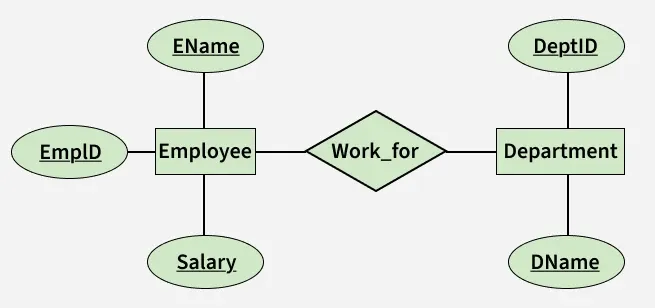
\includegraphics[width=\textwidth,height=0.78\textheight,keepaspectratio]{images/enhanced-er-model-relationship.png}
\end{frame}

%------------------------------------------------
\begin{frame}{Quiz nhanh: Giới thiệu tổng quan}
\textbf{Câu 1.} EER Model được dùng chủ yếu để làm gì?
\begin{enumerate}[A.]
    \item Biểu diễn các yêu cầu dữ liệu phức tạp hơn ER Model cơ bản
    \item Thay thế hoàn toàn SQL
    \item Tối ưu tốc độ truy vấn vật lý
    \item Sao lưu dữ liệu tự động
\end{enumerate}
\vspace{0.2cm}
\textbf{Câu 2.} Khái niệm nào sau đây thuộc EER Model?
\begin{enumerate}[A.]
    \item File system
    \item Packet switching
    \item Superclass và subclass
    \item Deadlock detection
\end{enumerate}
\end{frame}

\section{Superclass, Subclass và Inheritance}

%------------------------------------------------
\begin{frame}{Superclass}
\begin{block}{Khái niệm}
\concept{Superclass} là entity set tổng quát, chứa các thuộc tính chung của nhiều nhóm thực thể con.
\end{block}

\textbf{Ví dụ:}
\begin{center}
\codeword{Employee(eno, name, salary)}
\end{center}

\begin{itemize}
    \item \codeword{Employee} là superclass.
    \item Mọi loại nhân viên đều có mã, tên và lương.
    \item Thuộc tính chung được đặt ở mức tổng quát để tránh lặp lại.
\end{itemize}
\end{frame}

%------------------------------------------------
\begin{frame}{Subclass}
\begin{block}{Khái niệm}
\concept{Subclass} là entity set chuyên biệt hơn, kế thừa thuộc tính và quan hệ từ superclass, đồng thời có thể có thuộc tính riêng.
\end{block}

\textbf{Ví dụ:}
\begin{center}
\codeword{Secretary(typing\_speed)}\quad
\codeword{Technician(skill)}\quad
\codeword{Engineer(trade)}
\end{center}

\begin{itemize}
    \item Mỗi subclass là một loại cụ thể của \codeword{Employee}.
    \item Subclass kế thừa \codeword{eno}, \codeword{name}, \codeword{salary}.
    \item Subclass có thể bổ sung thuộc tính riêng.
\end{itemize}
\end{frame}

%------------------------------------------------
\begin{frame}{Minh họa superclass và subclass}
\centering
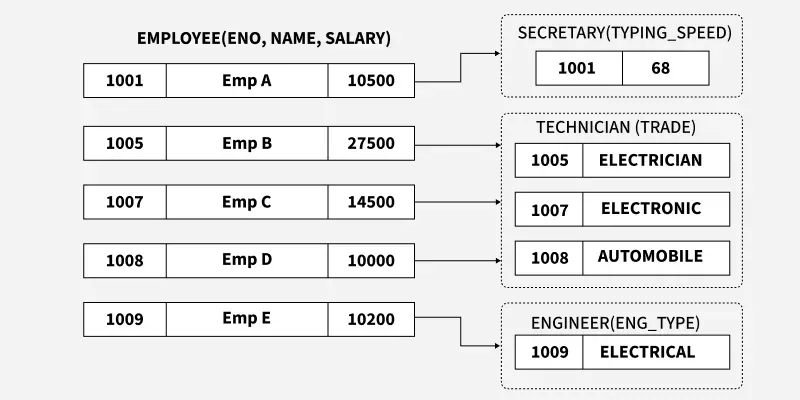
\includegraphics[width=\textwidth,height=0.78\textheight,keepaspectratio]{images/enhanced-er-model-3.png}
\end{frame}

%------------------------------------------------
\begin{frame}{Inheritance trong EER}
\begin{block}{Khái niệm}
\concept{Inheritance} nghĩa là subclass kế thừa thuộc tính và quan hệ của superclass.
\end{block}

Nếu \codeword{Engineer} là subclass của \codeword{Employee}, thì \codeword{Engineer} có:
\begin{itemize}
    \item Thuộc tính chung: \codeword{eno}, \codeword{name}, \codeword{salary}.
    \item Thuộc tính riêng: \codeword{trade}.
    \item Các relationship mà \codeword{Employee} tham gia, nếu phù hợp về nghiệp vụ.
\end{itemize}

\begin{alertblock}{Lưu ý}
Không nên tạo subclass nếu subclass không có thuộc tính riêng, quan hệ riêng hoặc quy tắc nghiệp vụ riêng.
\end{alertblock}
\end{frame}

%------------------------------------------------
\begin{frame}{Quiz nhanh: Khái niệm cơ bản}
\textbf{Câu 1.} Superclass là gì?
\begin{enumerate}[A.]
    \item Một bảng chỉ chứa khóa ngoại
    \item Entity set tổng quát chứa các thuộc tính chung
    \item Một thuộc tính đa trị
    \item Một quan hệ không có cardinality
\end{enumerate}
\vspace{0.2cm}
\textbf{Câu 2.} Subclass có đặc điểm nào?
\begin{enumerate}[A.]
    \item Không liên quan đến superclass
    \item Chỉ dùng trong mô hình vật lý
    \item Kế thừa thuộc tính và quan hệ từ superclass
    \item Không thể có thuộc tính riêng
\end{enumerate}
\end{frame}

\section{Quy trình mô hình hóa EER}

%------------------------------------------------
\begin{frame}{EER Model hoạt động như thế nào?}
EER Model bổ sung các cơ chế trừu tượng hóa vào ER Model cơ bản.

\vspace{0.3cm}
\begin{enumerate}
    \item \textbf{Xác định entity tổng quát}: tìm nhóm thực thể có thuộc tính chung.
    \item \textbf{Xác định entity chuyên biệt}: tìm nhóm con có thuộc tính hoặc quan hệ riêng.
    \item \textbf{Xác định ràng buộc}: total/partial và disjoint/overlapping.
    \item \textbf{Chuyển sang mô hình quan hệ}: chọn chiến lược mapping phù hợp.
\end{enumerate}

\vspace{0.2cm}
\begin{center}
\codeword{Employee -> Secretary, Technician, Engineer}
\end{center}
\end{frame}

%------------------------------------------------
\begin{frame}{Quy trình mô hình hóa EER}
\centering
\begin{tikzpicture}[
    node distance=1.1cm,
    processstep/.style={rectangle, rounded corners, draw=NEUBlue, thick, fill=NEULight, minimum width=3.3cm, minimum height=0.7cm, align=center},
    arrow/.style={-{Stealth[length=2.5mm]}, thick, color=NEUBlue}
]
\node[processstep] (s1) {1. Entity tổng quát};
\node[processstep, below=of s1] (s2) {2. Entity chuyên biệt};
\node[processstep, below=of s2] (s3) {3. Ràng buộc subclass};
\node[processstep, below=of s3] (s4) {4. Mapping sang quan hệ};
\draw[arrow] (s1) -- (s2);
\draw[arrow] (s2) -- (s3);
\draw[arrow] (s3) -- (s4);
\end{tikzpicture}
\end{frame}

%------------------------------------------------
\begin{frame}{Quiz nhanh: Cách hoạt động}
\textbf{Câu 1.} Bước đầu tiên khi mô hình hóa EER thường là gì?
\begin{enumerate}[A.]
    \item Xác định entity tổng quát và các thuộc tính chung
    \item Xóa toàn bộ relationship
    \item Viết truy vấn \codeword{SELECT}
    \item Tạo index vật lý
\end{enumerate}
\vspace{0.2cm}
\textbf{Câu 2.} Vì sao cần xác định ràng buộc subclass?
\begin{enumerate}[A.]
    \item Để bỏ qua khóa chính
    \item Để mô hình phản ánh đúng quy tắc nghiệp vụ
    \item Để không cần dùng entity
    \item Để thay thế database server
\end{enumerate}
\end{frame}

\section{Generalization và Specialization}

%------------------------------------------------
\begin{frame}{Generalization}
\begin{block}{Khái niệm}
\concept{Generalization} là quá trình gom nhiều entity set chuyên biệt thành một entity set tổng quát hơn.
\end{block}

\textbf{Ví dụ:}
\begin{center}
\codeword{Car, Truck, Motorbike -> Vehicle}
\end{center}

\begin{itemize}
    \item Thường đi từ dưới lên.
    \item Tập trung vào thuộc tính chung.
    \item Giúp giảm trùng lặp trong mô hình.
\end{itemize}
\end{frame}

%------------------------------------------------
\begin{frame}{Specialization}
\begin{block}{Khái niệm}
\concept{Specialization} là quá trình chia một entity set tổng quát thành các entity set chuyên biệt hơn.
\end{block}

\textbf{Ví dụ:}
\begin{center}
\codeword{Employee -> Secretary, Technician, Engineer}
\end{center}

\begin{itemize}
    \item Thường đi từ trên xuống.
    \item Tập trung vào đặc điểm riêng của từng subclass.
    \item Làm rõ quy tắc nghiệp vụ của từng nhóm thực thể.
\end{itemize}
\end{frame}

%------------------------------------------------
\begin{frame}{So sánh generalization và specialization}
\begin{table}
\centering
\small
\begin{tabularx}{\textwidth}{>{\bfseries}lXX}
\toprule
Tiêu chí & Generalization & Specialization \\
\midrule
Hướng phân tích & Từ dưới lên & Từ trên xuống \\
Ý tưởng & Gom các entity chuyên biệt & Chia entity tổng quát \\
Mục tiêu & Tìm thuộc tính chung & Tìm thuộc tính riêng \\
Ví dụ & Car, Truck -> Vehicle & Employee -> Engineer \\
\bottomrule
\end{tabularx}
\end{table}
\end{frame}

%------------------------------------------------
\begin{frame}{Minh họa generalization/specialization}
\centering
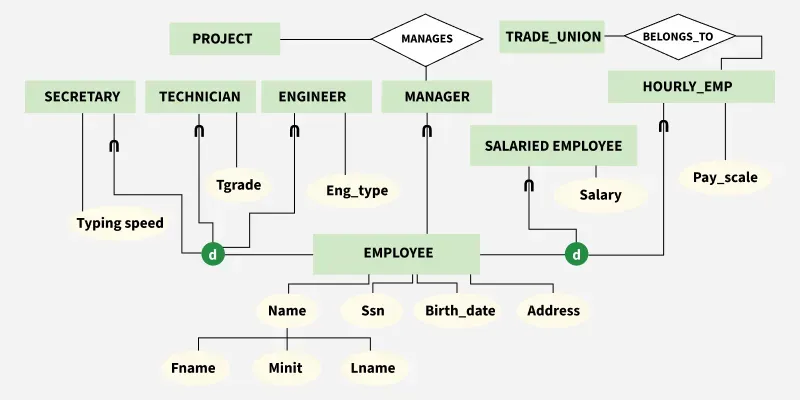
\includegraphics[width=\textwidth,height=0.78\textheight,keepaspectratio]{images/enhanced-er-model-1.png}
\end{frame}

%------------------------------------------------
\begin{frame}{Quiz nhanh: Generalization và specialization}
\textbf{Câu 1.} \codeword{Car}, \codeword{Truck}, \codeword{Motorbike} được gom thành \codeword{Vehicle} là ví dụ của gì?
\begin{enumerate}[A.]
    \item Aggregation
    \item Deadlock
    \item Generalization
    \item Fragmentation
\end{enumerate}
\vspace{0.2cm}
\textbf{Câu 2.} \codeword{Employee} được chia thành \codeword{Secretary}, \codeword{Technician}, \codeword{Engineer} là ví dụ của gì?
\begin{enumerate}[A.]
    \item Backup
    \item Indexing
    \item Transaction logging
    \item Specialization
\end{enumerate}
\end{frame}

\section{Ràng buộc subclassing}

%------------------------------------------------
\begin{frame}{Các ràng buộc trong specialization}
Các ràng buộc subclassing giúp xác định cách một thực thể của superclass tham gia vào các subclass.

\vspace{0.3cm}
\begin{columns}
\column{0.48\textwidth}
\begin{block}{Theo mức độ bao phủ}
\begin{itemize}
    \item Total subclassing.
    \item Partial subclassing.
\end{itemize}
\end{block}

\column{0.48\textwidth}
\begin{block}{Theo mức độ giao nhau}
\begin{itemize}
    \item Disjoint subclassing.
    \item Overlapping subclassing.
\end{itemize}
\end{block}
\end{columns}
\end{frame}

%------------------------------------------------
\begin{frame}{Total và partial subclassing}
\begin{block}{Total subclassing}
Mọi thực thể trong superclass bắt buộc phải thuộc ít nhất một subclass.
\end{block}
\textbf{Ví dụ:} mọi \codeword{Account} phải là \codeword{SavingsAccount} hoặc \codeword{CurrentAccount}.

\vspace{0.3cm}
\begin{block}{Partial subclassing}
Một số thực thể trong superclass có thể không thuộc subclass nào.
\end{block}
\textbf{Ví dụ:} không phải mọi \codeword{Employee} đều là \codeword{Secretary}, \codeword{Technician} hoặc \codeword{Engineer}.
\end{frame}

%------------------------------------------------
\begin{frame}{Disjoint và overlapping subclassing}
\begin{block}{Disjoint subclassing}
Một thực thể chỉ được thuộc tối đa một subclass.
\end{block}
\textbf{Ví dụ:} một tài khoản chỉ là \codeword{SavingsAccount} hoặc \codeword{CurrentAccount}.

\vspace{0.3cm}
\begin{block}{Overlapping subclassing}
Một thực thể có thể thuộc nhiều subclass cùng lúc.
\end{block}
\textbf{Ví dụ:} một nhân viên có thể vừa là \codeword{Teacher}, vừa là \codeword{Researcher}.
\end{frame}

%------------------------------------------------
\begin{frame}{Bảng so sánh ràng buộc subclassing}
\begin{table}
\centering
\scriptsize
\begin{tabularx}{\textwidth}{>{\bfseries}lXX}
\toprule
Ràng buộc & Ý nghĩa & Ví dụ \\
\midrule
Total & Mọi superclass entity phải thuộc subclass & Account -> Savings/Current \\
Partial & Có entity không thuộc subclass nào & Employee không nhất thiết là Engineer \\
Disjoint & Một entity thuộc tối đa một subclass & Tài khoản chỉ thuộc một loại \\
Overlapping & Một entity thuộc nhiều subclass & Teacher và Researcher \\
\bottomrule
\end{tabularx}
\end{table}
\end{frame}

%------------------------------------------------
\begin{frame}{Quiz nhanh: Ràng buộc subclassing}
\textbf{Câu 1.} Total subclassing nghĩa là gì?
\begin{enumerate}[A.]
    \item Không entity nào thuộc subclass
    \item Một entity chỉ có đúng một thuộc tính
    \item Mọi entity trong superclass phải thuộc ít nhất một subclass
    \item Mọi subclass đều không có thuộc tính riêng
\end{enumerate}
\vspace{0.2cm}
\textbf{Câu 2.} Disjoint subclassing mô tả trường hợp nào?
\begin{enumerate}[A.]
    \item Một entity chỉ được thuộc tối đa một subclass
    \item Một entity bắt buộc thuộc nhiều subclass
    \item Một subclass không có khóa chính
    \item Một relationship không có cardinality
\end{enumerate}
\end{frame}

\section{Aggregation và Category}

%------------------------------------------------
\begin{frame}{Aggregation}
\begin{block}{Khái niệm}
\concept{Aggregation} là cơ chế xem một relationship cùng các entity liên quan như một thực thể cấp cao hơn.
\end{block}

Aggregation hữu ích khi:
\begin{itemize}
    \item Một relationship cần tham gia vào relationship khác.
    \item Cần mô hình hóa ``relationship của relationship''.
    \item Cần biểu diễn nghiệp vụ ở mức trừu tượng cao hơn.
\end{itemize}
\end{frame}

%------------------------------------------------
\begin{frame}{Category hoặc union type}
\begin{block}{Khái niệm}
\concept{Category} hay \concept{union type} là một subclass được hình thành từ nhiều superclass khác nhau.
\end{block}

\textbf{Ví dụ:}
\begin{itemize}
    \item \codeword{LibraryMember} có thể là \codeword{Student}, \codeword{Faculty} hoặc \codeword{Staff}.
    \item \codeword{VehicleOwner} có thể là \codeword{Person} hoặc \codeword{Company}.
\end{itemize}
\end{frame}

%------------------------------------------------
\begin{frame}{Minh họa category/union type}
\centering
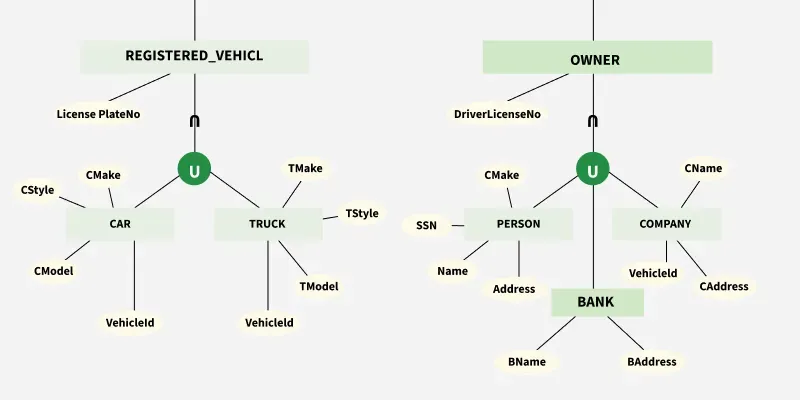
\includegraphics[width=\textwidth,height=0.78\textheight,keepaspectratio]{images/enhanced-er-model-2.png}
\end{frame}

%------------------------------------------------
\begin{frame}{Quiz nhanh: Category và aggregation}
\textbf{Câu 1.} \codeword{LibraryMember} là union của \codeword{Student}, \codeword{Faculty}, \codeword{Staff} là ví dụ của gì?
\begin{enumerate}[A.]
    \item Weak entity
    \item Category
    \item Derived attribute
    \item Index
\end{enumerate}
\vspace{0.2cm}
\textbf{Câu 2.} Aggregation hữu ích khi nào?
\begin{enumerate}[A.]
    \item Khi không có entity nào
    \item Khi chỉ có một thuộc tính
    \item Khi cần xem một relationship như một đối tượng cấp cao hơn
    \item Khi muốn bỏ qua nghiệp vụ
\end{enumerate}
\end{frame}

\section{Mapping EER sang mô hình quan hệ}

%------------------------------------------------
\begin{frame}{Vì sao cần mapping EER sang quan hệ?}
EER là mô hình khái niệm, còn cơ sở dữ liệu quan hệ cần các bảng cụ thể.

\vspace{0.3cm}
Khi chuyển EER sang mô hình quan hệ, cần quyết định:
\begin{itemize}
    \item Tạo bảng nào?
    \item Khóa chính và khóa ngoại nằm ở đâu?
    \item Thuộc tính chung và thuộc tính riêng được lưu thế nào?
    \item Cách biểu diễn total/partial và disjoint/overlapping ra sao?
\end{itemize}
\end{frame}

%------------------------------------------------
\begin{frame}{Một số chiến lược mapping phổ biến}
\begin{enumerate}
    \item \textbf{Một bảng cho superclass và mỗi subclass}
    \begin{itemize}
        \item Superclass lưu thuộc tính chung.
        \item Subclass lưu thuộc tính riêng và khóa ngoại về superclass.
    \end{itemize}
    \item \textbf{Một bảng duy nhất cho toàn bộ phân cấp}
    \begin{itemize}
        \item Thêm cột phân loại, ví dụ \codeword{employee\_type}.
    \end{itemize}
    \item \textbf{Chỉ tạo bảng cho subclass}
    \begin{itemize}
        \item Phù hợp trong một số trường hợp total và disjoint.
    \end{itemize}
\end{enumerate}
\end{frame}

%------------------------------------------------
\begin{frame}[fragile]{Ví dụ mapping: bảng superclass và subclass}
\begin{lstlisting}
CREATE TABLE Employee (
    eno INT PRIMARY KEY,
    name VARCHAR(100),
    salary DECIMAL(12,2)
);

CREATE TABLE Engineer (
    eno INT PRIMARY KEY,
    trade VARCHAR(100),
    FOREIGN KEY (eno) REFERENCES Employee(eno)
);
\end{lstlisting}
\end{frame}

%------------------------------------------------
\begin{frame}[fragile]{Ví dụ mapping: một bảng duy nhất}
\begin{lstlisting}
CREATE TABLE Employee (
    eno INT PRIMARY KEY,
    name VARCHAR(100),
    salary DECIMAL(12,2),
    employee_type VARCHAR(30),
    typing_speed INT,
    skill VARCHAR(100),
    trade VARCHAR(100)
);
\end{lstlisting}

\begin{alertblock}{Nhận xét}
Cách này đơn giản nhưng có thể tạo nhiều giá trị NULL nếu các subclass có nhiều thuộc tính riêng.
\end{alertblock}
\end{frame}

%------------------------------------------------
\begin{frame}{Nguyên tắc chọn chiến lược mapping}
\begin{itemize}
    \item Nếu cần mô hình rõ ràng và giảm NULL: dùng bảng riêng cho superclass/subclass.
    \item Nếu phân cấp đơn giản và truy vấn thường cần toàn bộ dữ liệu: có thể dùng một bảng duy nhất.
    \item Nếu total và disjoint rõ ràng: có thể cân nhắc chỉ tạo bảng cho subclass.
    \item Cần cân bằng giữa tính chuẩn hóa, hiệu năng truy vấn và độ phức tạp triển khai.
\end{itemize}
\end{frame}

\section{Ứng dụng và vai trò}

%------------------------------------------------
\begin{frame}{Ứng dụng thực tế của EER Model}
\begin{enumerate}
    \item \textbf{Quản lý nhân sự}: Employee và các loại nhân viên.
    \item \textbf{Ngân hàng}: Account và các loại tài khoản.
    \item \textbf{Giao thông}: Vehicle và các loại phương tiện.
    \item \textbf{Thư viện}: LibraryMember là union của Student, Faculty, Staff.
    \item \textbf{Giáo dục}: một người có thể vừa là Teacher vừa là Researcher.
\end{enumerate}
\end{frame}

%------------------------------------------------
\begin{frame}{Vai trò trong phân tích và thiết kế}
\begin{columns}
\column{0.5\textwidth}
\begin{block}{Phân tích nghiệp vụ}
\begin{itemize}
    \item Làm rõ nhóm đối tượng.
    \item Phản ánh quy tắc phân loại.
    \item Hỗ trợ trao đổi với stakeholder.
\end{itemize}
\end{block}

\column{0.5\textwidth}
\begin{block}{Thiết kế cơ sở dữ liệu}
\begin{itemize}
    \item Chọn chiến lược mapping.
    \item Giảm trùng lặp thuộc tính.
    \item Chuẩn hóa mô hình dữ liệu.
\end{itemize}
\end{block}
\end{columns}
\end{frame}

%------------------------------------------------
\begin{frame}{Vai trò trong phát triển phần mềm và quản trị dữ liệu}
\begin{columns}
\column{0.5\textwidth}
\begin{block}{Phát triển phần mềm}
\begin{itemize}
    \item Hỗ trợ domain model.
    \item Gần với khái niệm kế thừa nghiệp vụ.
    \item Giúp thiết kế API/schema nhất quán.
\end{itemize}
\end{block}

\column{0.5\textwidth}
\begin{block}{Quản trị dữ liệu}
\begin{itemize}
    \item Chuẩn hóa phân loại dữ liệu.
    \item Kiểm soát ràng buộc.
    \item Tài liệu hóa mô hình dữ liệu.
\end{itemize}
\end{block}
\end{columns}
\end{frame}

%------------------------------------------------
\begin{frame}{So sánh ER Model và Enhanced ER Model}
\begin{table}
\centering
\small
\begin{tabularx}{\textwidth}{>{\bfseries}lXX}
\toprule
Tiêu chí & ER Model & Enhanced ER Model \\
\midrule
Mức độ biểu diễn & Cơ bản & Nâng cao \\
Thành phần chính & Entity, attribute, relationship & Thêm superclass, subclass, inheritance, category, aggregation \\
Phân cấp & Hạn chế & Tốt \\
Kế thừa & Không trực tiếp & Có \\
Phù hợp với & Bài toán đơn giản & Bài toán phức tạp, nhiều loại thực thể \\
\bottomrule
\end{tabularx}
\end{table}
\end{frame}

%------------------------------------------------
\begin{frame}{Quiz nhanh: Ứng dụng và vai trò}
\textbf{Câu 1.} Hệ thống nào thường cần EER Model?
\begin{enumerate}[A.]
    \item Hệ thống chỉ có một biến số
    \item Hệ thống không có dữ liệu
    \item Hệ thống không cần mô hình hóa
    \item Hệ thống có nhiều loại thực thể phân cấp
\end{enumerate}
\vspace{0.2cm}
\textbf{Câu 2.} Trong thiết kế database, EER giúp gì?
\begin{enumerate}[A.]
    \item Tăng tốc CPU
    \item Tạo giao diện web
    \item Cài đặt hệ điều hành
    \item Chọn chiến lược mapping superclass/subclass
\end{enumerate}
\end{frame}

\section{Câu hỏi và bài tập}

%------------------------------------------------
\begin{frame}{Câu hỏi ôn tập trắc nghiệm 1}
\textbf{Câu 1.} EER Model là gì?
\begin{enumerate}[A.]
    \item Một hệ quản trị cơ sở dữ liệu
    \item Mô hình ER mở rộng để biểu diễn yêu cầu dữ liệu phức tạp hơn
    \item Một ngôn ngữ lập trình
    \item Một dạng file sao lưu
\end{enumerate}

\vspace{0.2cm}
\textbf{Câu 2.} Superclass trong EER Model có vai trò gì?
\begin{enumerate}[A.]
    \item Chỉ chứa dữ liệu tạm thời
    \item Chỉ dùng để biểu diễn khóa ngoại
    \item Chứa các thuộc tính chung của nhiều subclass
    \item Không liên quan đến subclass
\end{enumerate}
\end{frame}

%------------------------------------------------
\begin{frame}{Câu hỏi ôn tập trắc nghiệm 2}
\textbf{Câu 3.} Subclass kế thừa gì từ superclass?
\begin{enumerate}[A.]
    \item Chỉ tên bảng
    \item Chỉ dữ liệu mẫu
    \item Chỉ câu lệnh SQL
    \item Thuộc tính và quan hệ
\end{enumerate}

\vspace{0.2cm}
\textbf{Câu 4.} Generalization là quá trình nào?
\begin{enumerate}[A.]
    \item Gom các entity chuyên biệt thành entity tổng quát
    \item Chia entity tổng quát thành các entity chuyên biệt
    \item Xóa toàn bộ relationship
    \item Tạo chỉ mục cho bảng
\end{enumerate}
\end{frame}

%------------------------------------------------
\begin{frame}{Câu hỏi tự luận ngắn}
\begin{enumerate}
    \item Trình bày khái niệm Enhanced ER Model.
    \item Giải thích vai trò của superclass và subclass.
    \item Phân biệt generalization và specialization.
    \item Phân biệt total subclassing và partial subclassing.
    \item Phân biệt disjoint subclassing và overlapping subclassing.
\end{enumerate}
\end{frame}

%------------------------------------------------
\begin{frame}{Bài tập vận dụng 1}
\begin{block}{Tình huống}
Một hệ thống nhân sự có entity \codeword{Employee}. Nhân viên có thể được phân thành \codeword{Secretary}, \codeword{Technician} và \codeword{Engineer}.
\end{block}

\textbf{Yêu cầu:}
\begin{itemize}
    \item Xác định superclass và subclass.
    \item Đề xuất thuộc tính chung.
    \item Đề xuất thuộc tính riêng cho từng subclass.
\end{itemize}
\end{frame}

%------------------------------------------------
\begin{frame}{Bài tập vận dụng 2}
\begin{block}{Tình huống}
Một trường đại học có nhân sự vừa có thể là \codeword{Teacher}, vừa có thể là \codeword{Researcher}.
\end{block}

\textbf{Yêu cầu:}
\begin{itemize}
    \item Xác định đây là disjoint hay overlapping subclassing.
    \item Giải thích lý do.
    \item Gợi ý cách biểu diễn trong mô hình EER.
\end{itemize}
\end{frame}

%------------------------------------------------
\begin{frame}{Bài tập vận dụng 3}
\begin{block}{Tình huống}
Một thư viện có thành viên là \codeword{Student}, \codeword{Faculty} hoặc \codeword{Staff}.
\end{block}

\textbf{Yêu cầu:}
\begin{itemize}
    \item Thiết kế mô hình EER đơn giản.
    \item Biểu diễn \codeword{LibraryMember} là category hoặc union type.
    \item Đề xuất cách mapping sang mô hình quan hệ.
\end{itemize}
\end{frame}

\section{Tóm tắt và đáp án}

%------------------------------------------------
\begin{frame}{Tóm tắt bài học}
\begin{itemize}
    \item EER Model là phần mở rộng của ER Model truyền thống.
    \item EER giúp biểu diễn phân cấp, kế thừa và phân loại thực thể.
    \item Superclass chứa thuộc tính chung; subclass chứa thuộc tính riêng.
    \item Generalization gom entity chuyên biệt thành entity tổng quát.
    \item Specialization chia entity tổng quát thành entity chuyên biệt.
    \item Total/partial mô tả mức độ bao phủ.
    \item Disjoint/overlapping mô tả khả năng thuộc một hoặc nhiều subclass.
    \item Category/union type biểu diễn subclass từ nhiều superclass.
\end{itemize}
\end{frame}

%------------------------------------------------
\begin{frame}{Từ khóa chính}
\begin{multicols}{2}
\begin{itemize}
    \item Enhanced ER Model
    \item EER Model
    \item ER Model
    \item Superclass
    \item Subclass
    \item Inheritance
    \item Generalization
    \item Specialization
    \item Total subclassing
    \item Partial subclassing
    \item Disjoint subclassing
    \item Overlapping subclassing
    \item Category
    \item Union type
    \item Aggregation
\end{itemize}
\end{multicols}
\end{frame}

%------------------------------------------------
\begin{frame}{Đáp án quiz nhanh}
\scriptsize
\begin{tabularx}{\textwidth}{>{\bfseries}lX}
\toprule
Nhóm câu hỏi & Đáp án \\
\midrule
Giới thiệu tổng quan & Câu 1: A; Câu 2: C \\
Khái niệm cơ bản & Câu 1: B; Câu 2: C \\
Cách hoạt động & Câu 1: A; Câu 2: B \\
Generalization/Specialization & Câu 1: C; Câu 2: D \\
Ràng buộc subclassing & Câu 1: C; Câu 2: A \\
Category/Aggregation & Câu 1: B; Câu 2: C \\
Ứng dụng/Vai trò & Câu 1: D; Câu 2: D \\
\bottomrule
\end{tabularx}
\end{frame}

%------------------------------------------------
\begin{frame}{Đáp án câu hỏi ôn tập}
\begin{itemize}
    \item \textbf{Câu 1:} B.
    \item \textbf{Câu 2:} C.
    \item \textbf{Câu 3:} D.
    \item \textbf{Câu 4:} A.
\end{itemize}

\begin{block}{Gợi ý tự luận}
Cần nhấn mạnh các ý: EER là ER mở rộng; superclass lưu thuộc tính chung; subclass kế thừa và có thể có thuộc tính riêng; generalization đi từ dưới lên; specialization đi từ trên xuống.
\end{block}
\end{frame}

%------------------------------------------------
\begin{frame}{Gợi ý bài tập vận dụng}
\begin{itemize}
    \item \textbf{Bài 1:} Superclass là \codeword{Employee}; subclass là \codeword{Secretary}, \codeword{Technician}, \codeword{Engineer}. Thuộc tính riêng: \codeword{typing\_speed}, \codeword{skill}, \codeword{trade}.
    \item \textbf{Bài 2:} Đây là overlapping subclassing vì một nhân sự có thể đồng thời là \codeword{Teacher} và \codeword{Researcher}.
    \item \textbf{Bài 3:} \codeword{LibraryMember} là category/union type được hình thành từ \codeword{Student}, \codeword{Faculty}, \codeword{Staff}.
\end{itemize}
\end{frame}

%------------------------------------------------
\begin{frame}
\centering
\Huge Cảm ơn!\\[0.5cm]
\Large Câu hỏi và thảo luận
\end{frame}

\end{document}
